% Generated by Sphinx.
\def\sphinxdocclass{report}
\documentclass[letterpaper,10pt,english]{sphinxmanual}
\usepackage[utf8]{inputenc}
\DeclareUnicodeCharacter{00A0}{\nobreakspace}
\usepackage[T1]{fontenc}
\usepackage{babel}
\usepackage{times}
\usepackage[Bjarne]{fncychap}
\usepackage{longtable}
\usepackage{sphinx}
\usepackage{multirow}


\title{Juju docs - Sphinx Edition Documentation}
\date{December 05, 2013}
\release{0.1}
\author{Winael}
\newcommand{\sphinxlogo}{}
\renewcommand{\releasename}{Release}
\makeindex

\makeatletter
\def\PYG@reset{\let\PYG@it=\relax \let\PYG@bf=\relax%
    \let\PYG@ul=\relax \let\PYG@tc=\relax%
    \let\PYG@bc=\relax \let\PYG@ff=\relax}
\def\PYG@tok#1{\csname PYG@tok@#1\endcsname}
\def\PYG@toks#1+{\ifx\relax#1\empty\else%
    \PYG@tok{#1}\expandafter\PYG@toks\fi}
\def\PYG@do#1{\PYG@bc{\PYG@tc{\PYG@ul{%
    \PYG@it{\PYG@bf{\PYG@ff{#1}}}}}}}
\def\PYG#1#2{\PYG@reset\PYG@toks#1+\relax+\PYG@do{#2}}

\expandafter\def\csname PYG@tok@gd\endcsname{\def\PYG@tc##1{\textcolor[rgb]{0.63,0.00,0.00}{##1}}}
\expandafter\def\csname PYG@tok@gu\endcsname{\let\PYG@bf=\textbf\def\PYG@tc##1{\textcolor[rgb]{0.50,0.00,0.50}{##1}}}
\expandafter\def\csname PYG@tok@gt\endcsname{\def\PYG@tc##1{\textcolor[rgb]{0.00,0.27,0.87}{##1}}}
\expandafter\def\csname PYG@tok@gs\endcsname{\let\PYG@bf=\textbf}
\expandafter\def\csname PYG@tok@gr\endcsname{\def\PYG@tc##1{\textcolor[rgb]{1.00,0.00,0.00}{##1}}}
\expandafter\def\csname PYG@tok@cm\endcsname{\let\PYG@it=\textit\def\PYG@tc##1{\textcolor[rgb]{0.25,0.50,0.56}{##1}}}
\expandafter\def\csname PYG@tok@vg\endcsname{\def\PYG@tc##1{\textcolor[rgb]{0.73,0.38,0.84}{##1}}}
\expandafter\def\csname PYG@tok@m\endcsname{\def\PYG@tc##1{\textcolor[rgb]{0.13,0.50,0.31}{##1}}}
\expandafter\def\csname PYG@tok@mh\endcsname{\def\PYG@tc##1{\textcolor[rgb]{0.13,0.50,0.31}{##1}}}
\expandafter\def\csname PYG@tok@cs\endcsname{\def\PYG@tc##1{\textcolor[rgb]{0.25,0.50,0.56}{##1}}\def\PYG@bc##1{\setlength{\fboxsep}{0pt}\colorbox[rgb]{1.00,0.94,0.94}{\strut ##1}}}
\expandafter\def\csname PYG@tok@ge\endcsname{\let\PYG@it=\textit}
\expandafter\def\csname PYG@tok@vc\endcsname{\def\PYG@tc##1{\textcolor[rgb]{0.73,0.38,0.84}{##1}}}
\expandafter\def\csname PYG@tok@il\endcsname{\def\PYG@tc##1{\textcolor[rgb]{0.13,0.50,0.31}{##1}}}
\expandafter\def\csname PYG@tok@go\endcsname{\def\PYG@tc##1{\textcolor[rgb]{0.20,0.20,0.20}{##1}}}
\expandafter\def\csname PYG@tok@cp\endcsname{\def\PYG@tc##1{\textcolor[rgb]{0.00,0.44,0.13}{##1}}}
\expandafter\def\csname PYG@tok@gi\endcsname{\def\PYG@tc##1{\textcolor[rgb]{0.00,0.63,0.00}{##1}}}
\expandafter\def\csname PYG@tok@gh\endcsname{\let\PYG@bf=\textbf\def\PYG@tc##1{\textcolor[rgb]{0.00,0.00,0.50}{##1}}}
\expandafter\def\csname PYG@tok@ni\endcsname{\let\PYG@bf=\textbf\def\PYG@tc##1{\textcolor[rgb]{0.84,0.33,0.22}{##1}}}
\expandafter\def\csname PYG@tok@nl\endcsname{\let\PYG@bf=\textbf\def\PYG@tc##1{\textcolor[rgb]{0.00,0.13,0.44}{##1}}}
\expandafter\def\csname PYG@tok@nn\endcsname{\let\PYG@bf=\textbf\def\PYG@tc##1{\textcolor[rgb]{0.05,0.52,0.71}{##1}}}
\expandafter\def\csname PYG@tok@no\endcsname{\def\PYG@tc##1{\textcolor[rgb]{0.38,0.68,0.84}{##1}}}
\expandafter\def\csname PYG@tok@na\endcsname{\def\PYG@tc##1{\textcolor[rgb]{0.25,0.44,0.63}{##1}}}
\expandafter\def\csname PYG@tok@nb\endcsname{\def\PYG@tc##1{\textcolor[rgb]{0.00,0.44,0.13}{##1}}}
\expandafter\def\csname PYG@tok@nc\endcsname{\let\PYG@bf=\textbf\def\PYG@tc##1{\textcolor[rgb]{0.05,0.52,0.71}{##1}}}
\expandafter\def\csname PYG@tok@nd\endcsname{\let\PYG@bf=\textbf\def\PYG@tc##1{\textcolor[rgb]{0.33,0.33,0.33}{##1}}}
\expandafter\def\csname PYG@tok@ne\endcsname{\def\PYG@tc##1{\textcolor[rgb]{0.00,0.44,0.13}{##1}}}
\expandafter\def\csname PYG@tok@nf\endcsname{\def\PYG@tc##1{\textcolor[rgb]{0.02,0.16,0.49}{##1}}}
\expandafter\def\csname PYG@tok@si\endcsname{\let\PYG@it=\textit\def\PYG@tc##1{\textcolor[rgb]{0.44,0.63,0.82}{##1}}}
\expandafter\def\csname PYG@tok@s2\endcsname{\def\PYG@tc##1{\textcolor[rgb]{0.25,0.44,0.63}{##1}}}
\expandafter\def\csname PYG@tok@vi\endcsname{\def\PYG@tc##1{\textcolor[rgb]{0.73,0.38,0.84}{##1}}}
\expandafter\def\csname PYG@tok@nt\endcsname{\let\PYG@bf=\textbf\def\PYG@tc##1{\textcolor[rgb]{0.02,0.16,0.45}{##1}}}
\expandafter\def\csname PYG@tok@nv\endcsname{\def\PYG@tc##1{\textcolor[rgb]{0.73,0.38,0.84}{##1}}}
\expandafter\def\csname PYG@tok@s1\endcsname{\def\PYG@tc##1{\textcolor[rgb]{0.25,0.44,0.63}{##1}}}
\expandafter\def\csname PYG@tok@gp\endcsname{\let\PYG@bf=\textbf\def\PYG@tc##1{\textcolor[rgb]{0.78,0.36,0.04}{##1}}}
\expandafter\def\csname PYG@tok@sh\endcsname{\def\PYG@tc##1{\textcolor[rgb]{0.25,0.44,0.63}{##1}}}
\expandafter\def\csname PYG@tok@ow\endcsname{\let\PYG@bf=\textbf\def\PYG@tc##1{\textcolor[rgb]{0.00,0.44,0.13}{##1}}}
\expandafter\def\csname PYG@tok@sx\endcsname{\def\PYG@tc##1{\textcolor[rgb]{0.78,0.36,0.04}{##1}}}
\expandafter\def\csname PYG@tok@bp\endcsname{\def\PYG@tc##1{\textcolor[rgb]{0.00,0.44,0.13}{##1}}}
\expandafter\def\csname PYG@tok@c1\endcsname{\let\PYG@it=\textit\def\PYG@tc##1{\textcolor[rgb]{0.25,0.50,0.56}{##1}}}
\expandafter\def\csname PYG@tok@kc\endcsname{\let\PYG@bf=\textbf\def\PYG@tc##1{\textcolor[rgb]{0.00,0.44,0.13}{##1}}}
\expandafter\def\csname PYG@tok@c\endcsname{\let\PYG@it=\textit\def\PYG@tc##1{\textcolor[rgb]{0.25,0.50,0.56}{##1}}}
\expandafter\def\csname PYG@tok@mf\endcsname{\def\PYG@tc##1{\textcolor[rgb]{0.13,0.50,0.31}{##1}}}
\expandafter\def\csname PYG@tok@err\endcsname{\def\PYG@bc##1{\setlength{\fboxsep}{0pt}\fcolorbox[rgb]{1.00,0.00,0.00}{1,1,1}{\strut ##1}}}
\expandafter\def\csname PYG@tok@kd\endcsname{\let\PYG@bf=\textbf\def\PYG@tc##1{\textcolor[rgb]{0.00,0.44,0.13}{##1}}}
\expandafter\def\csname PYG@tok@ss\endcsname{\def\PYG@tc##1{\textcolor[rgb]{0.32,0.47,0.09}{##1}}}
\expandafter\def\csname PYG@tok@sr\endcsname{\def\PYG@tc##1{\textcolor[rgb]{0.14,0.33,0.53}{##1}}}
\expandafter\def\csname PYG@tok@mo\endcsname{\def\PYG@tc##1{\textcolor[rgb]{0.13,0.50,0.31}{##1}}}
\expandafter\def\csname PYG@tok@mi\endcsname{\def\PYG@tc##1{\textcolor[rgb]{0.13,0.50,0.31}{##1}}}
\expandafter\def\csname PYG@tok@kn\endcsname{\let\PYG@bf=\textbf\def\PYG@tc##1{\textcolor[rgb]{0.00,0.44,0.13}{##1}}}
\expandafter\def\csname PYG@tok@o\endcsname{\def\PYG@tc##1{\textcolor[rgb]{0.40,0.40,0.40}{##1}}}
\expandafter\def\csname PYG@tok@kr\endcsname{\let\PYG@bf=\textbf\def\PYG@tc##1{\textcolor[rgb]{0.00,0.44,0.13}{##1}}}
\expandafter\def\csname PYG@tok@s\endcsname{\def\PYG@tc##1{\textcolor[rgb]{0.25,0.44,0.63}{##1}}}
\expandafter\def\csname PYG@tok@kp\endcsname{\def\PYG@tc##1{\textcolor[rgb]{0.00,0.44,0.13}{##1}}}
\expandafter\def\csname PYG@tok@w\endcsname{\def\PYG@tc##1{\textcolor[rgb]{0.73,0.73,0.73}{##1}}}
\expandafter\def\csname PYG@tok@kt\endcsname{\def\PYG@tc##1{\textcolor[rgb]{0.56,0.13,0.00}{##1}}}
\expandafter\def\csname PYG@tok@sc\endcsname{\def\PYG@tc##1{\textcolor[rgb]{0.25,0.44,0.63}{##1}}}
\expandafter\def\csname PYG@tok@sb\endcsname{\def\PYG@tc##1{\textcolor[rgb]{0.25,0.44,0.63}{##1}}}
\expandafter\def\csname PYG@tok@k\endcsname{\let\PYG@bf=\textbf\def\PYG@tc##1{\textcolor[rgb]{0.00,0.44,0.13}{##1}}}
\expandafter\def\csname PYG@tok@se\endcsname{\let\PYG@bf=\textbf\def\PYG@tc##1{\textcolor[rgb]{0.25,0.44,0.63}{##1}}}
\expandafter\def\csname PYG@tok@sd\endcsname{\let\PYG@it=\textit\def\PYG@tc##1{\textcolor[rgb]{0.25,0.44,0.63}{##1}}}

\def\PYGZbs{\char`\\}
\def\PYGZus{\char`\_}
\def\PYGZob{\char`\{}
\def\PYGZcb{\char`\}}
\def\PYGZca{\char`\^}
\def\PYGZam{\char`\&}
\def\PYGZlt{\char`\<}
\def\PYGZgt{\char`\>}
\def\PYGZsh{\char`\#}
\def\PYGZpc{\char`\%}
\def\PYGZdl{\char`\$}
\def\PYGZhy{\char`\-}
\def\PYGZsq{\char`\'}
\def\PYGZdq{\char`\"}
\def\PYGZti{\char`\~}
% for compatibility with earlier versions
\def\PYGZat{@}
\def\PYGZlb{[}
\def\PYGZrb{]}
\makeatother

\begin{document}

\maketitle
\tableofcontents
\phantomsection\label{index::doc}


User Guide:


\chapter{Introduction}
\label{getting-started:introduction}\label{getting-started::doc}\label{getting-started:welcome-to-juju-docs-sphinx-edition-s-documentation}
This tutorial will show you how to get started with Juju, including
installing, configuring and bootstrapping a new Juju environment.
Before you start you will need:
\begin{itemize}
\item {} 
An Ubuntu, OSX or Windows machine to install the client on.

\item {} 
An environment which can provide a new server with an Ubuntu cloud
operating system image on-demand. This includes services such as
Amazon EC2, HP Cloud, an OpenStack installation, or your local machine

\item {} 
An SSH key-pair. If you have not already set one up, you need to
generate an appropriate keypair. On Linux and Mac OSX: \code{ssh-keygen -t
rsa -b 2048} On Windows: See the Windows instructions for SSH and
PuTTY

\end{itemize}


\chapter{Installation}
\label{getting-started:installation}
To install Juju, you simply need to grab the latest juju-core package
from the PPA:
\begin{itemize}
\item {} 
\textbf{Ubuntu :}

\begin{Verbatim}[commandchars=\\\{\}]
sudo add-apt-repository ppa:juju/stable
sudo apt-get update \&\& sudo apt-get install juju-core
\end{Verbatim}

\item {} 
\textbf{Mac OSX :}

Juju is in \href{http://brew.sh/}{Homebrew}, to install do:

\begin{Verbatim}[commandchars=\\\{\}]
brew install juju
\end{Verbatim}

\item {} 
\textbf{Windows :}

Download and run the \href{https://launchpad.net/juju-core/1.16/1.16.2/+download/juju-setup-1.16.2-signed.exe}{Juju windows installer from here.}

\end{itemize}


\chapter{Configuring}
\label{getting-started:configuring}
Now the Juju software is installed, it needs to be configured to use
your particular cloud provider. This is done by generating and editing
a file, \code{environments.yaml}, which will live in your \code{\textasciitilde{}/.juju/}
directory on Linux and OSX, \code{\%LOCALAPPDATA\%/Juju} on Windows. You can
generate the environments file manually, but Juju also includes a
boilerplate configuration option that will flesh out most of the file
for you and minimise the amount of work (and potential errors).

To generate an initial config file, you simply need to run:

\begin{Verbatim}[commandchars=\\\{\}]
juju generate-config
\end{Verbatim}

This command will cause a file to be written to your \textasciitilde{}/.juju directory
if an environments.yaml file does not already exist. It will also
create the \textasciitilde{}./juju directory if that does not exist.

This file will contain sample profiles for different types of cloud
services, but you will need to edit the files to provide specific
information for your cloud provider. Sections are created for Amazon
(AWS) services, HPCloud and a generic OpenStack instance (and for the
local provider if running on Linux). For more specifics on what needs
to be changed, see the relevant sections below.
\begin{itemize}
\item {} 
Configuring for Amazon AWS

\item {} 
\href{https://juju.ubuntu.com/config-azure.html}{Configuring for Windows Azure}

\item {} 
Configuring for HP Cloud

\item {} 
Configuring for OpenStack

\item {} 
Configuring for MAAS

\item {} 
\href{https://juju.ubuntu.com/config-local.html}{Configuring for LXC local provider (Linux)}

\end{itemize}


\chapter{Testing your setup}
\label{getting-started:testing-your-setup}
Once you have installed and configured Juju, it is probably a good
idea to take it for a bit of a test drive and check that everything is
working as expected. Because Juju makes it really easy to deploy
services, this is actually quick and straightforward.

The first thing to do is set up a bootstrap environment. This is an
instance in the cloud that Juju will use to deploy and control other
services with. It will be created according to the configuration you
have provided, and your SSH key will automatically be uploaded so that
Juju can communicate securely with the bootstrap instance.

\begin{Verbatim}[commandchars=\\\{\}]
juju bootstrap
\end{Verbatim}

\begin{notice}{note}{Note:}
If you have multiple environments configured, you can choose
which one to address with a particular command by adding the \code{-e}
switch followed by the environment name, E.g. \code{-e hpcloud}.
\end{notice}

You may have to wait a few moments for this command to return, as it
needs to perform various tasks and contact your cloud provider.

Assuming it returns successfully (otherwise see common error messages
and what to do about them), we can now deploy some services and
explore the basic operations of Juju.

To start with, we will deploy Wordpress, by running this command:

\begin{Verbatim}[commandchars=\\\{\}]
juju deploy wordpress
\end{Verbatim}

Now juju will fetch the Wordpress charm and use it, through the
bootstrap instance to request and deploy whatever resources it needs
to set up this service.

Wordpress needs a database though, so we will also deploy one of
those:

\begin{Verbatim}[commandchars=\\\{\}]
juju deploy mysql
\end{Verbatim}

Once again, juju will do whatever is necessary to deploy this service
for you, and it may take some time for the command to return.

\begin{notice}{note}{Note:}
If you want to get more information on what is actually
happening, or to help resolve problems, you can add the -v switch to
the juju command to get verbose output.
\end{notice}

Although we have deployed Wordpress and a MySQL database, they are not
linked together in any way yet. To do this we should run:

\begin{Verbatim}[commandchars=\\\{\}]
juju add-relation wordpress mysql
\end{Verbatim}

This command uses information provided by the relevant charms to
associate these services with each other in whatever way makes sense.
There is much more to be said about linking services together which is
covered in the juju command documentation, but for the moment, we just
need to know that it will link these services together.

In order to make our Wordpress public, we now need to expose this
service:

\begin{Verbatim}[commandchars=\\\{\}]
juju expose wordpress
\end{Verbatim}

This service will now be configured to respond to web requests, so
visitors can see it. But where exactly is it? If we run the juju
status command, we will be able to see what services are running, and
where they are located.

\begin{Verbatim}[commandchars=\\\{\}]
juju status
\end{Verbatim}

The output from this command should look something like this:

\begin{Verbatim}[commandchars=\\\{\}]
machines:
  "0":
    agent-state: started
    agent-version: 1.10.0
    dns-name: ec2-50-16-167-135.compute-1.amazonaws.com
    instance-id: i-781bf614
    series: precise
  "1":
    agent-state: started
    agent-version: 1.10.0
    dns-name: ec2-23-22-225-54.compute-1.amazonaws.com
    instance-id: i-9e8927f6
    series: precise
  "2":
    agent-state: started
    agent-version: 1.10.0
    dns-name: ec2-54-224-220-210.compute-1.amazonaws.com
    instance-id: i-5c440436
    series: precise
services:
  mysql:
    charm: cs:precise/mysql-18
    exposed: false
    relations:
      db:
      - wordpress
    units:
      mysql/0:
        agent-state: started
        agent-version: 1.10.0
        machine: "1"
        public-address: ec2-23-22-225-54.compute-1.amazonaws.com
  wordpress:
    charm: cs:precise/wordpress-12
    exposed: true
    relations:
      db:
      - mysql
      loadbalancer:
      - wordpress
    units:
      wordpress/0:
        agent-state: started
        agent-version: 1.10.0
        machine: "2"
        public-address: ec2-54-224-220-210.compute-1.amazonaws.com
\end{Verbatim}

There is quite a lot of information here. the first section, titled
machines: , details all the instances which are currently running. For
each you will see the version of Juju they are running, their
hostname, instance id and the series or version of Ubuntu they are
running.

After that, the sections list the services which are currently
deployed. The information here differs slightly according to the
service and how it is configured. It will however, always list the
charm that was used to deploy the service, whether it is exposed or
not, its address and whatever relationships exist.

From this status readout, we can see that wordpress is exposed and
ready. If we simply copy the address into a web browser, we should be
able to see it running

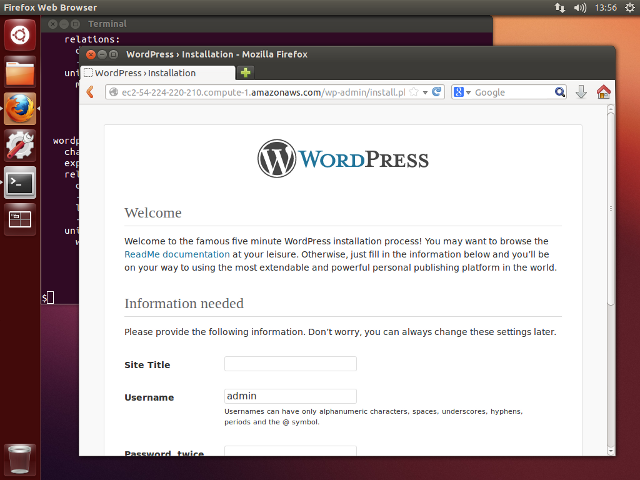
\includegraphics{getting_started-wordpress.png}

Congratulations, you have just deployed a service with Juju!

Now you are ready to deploy whatever service you really want from the
100s available at the \href{http://jujucharms.com}{Juju Charm Store.}

To remove all current deployments and clear up everything in your
cloud, you can run the command:

\begin{Verbatim}[commandchars=\\\{\}]
juju destroy-environment
\end{Verbatim}

This will remove everything, including the bootstrap node.

To learn more about charms, including configuring options and managing
running systems, you should continue to \href{https://juju.ubuntu.com/./charms.html}{read the charm
documentation.}


\chapter{Configuring for Amazon AWS}
\label{config-aws:configuring-for-amazon-aws}\label{config-aws::doc}\label{config-aws:is-covered-in-the-juju-command-documentation}
This process requires you to have an Amazon Web Services (AWS)
account. If you have not signed up for one yet, it can obtained at
\href{http://aws.amazon.com}{http://aws.amazon.com}.

You should start by generating a generic configuration file for Juju,
using the command:

\begin{Verbatim}[commandchars=\\\{\}]
juju generate-config
\end{Verbatim}

This will generate a file, environments.yaml , which will live in your
\textasciitilde{}/.juju/ directory (and will create the directory if it doesn't
already exist).

\begin{notice}{note}{Note:}
If you have an existing configuration, you can use \code{juju
generate-config -{-}show} to output the new config file, then copy and
paste relevant areas in a text editor etc.
\end{notice}

The generic configuration sections generated for AWS will look
something like this:

\begin{Verbatim}[commandchars=\\\{\}]
\#\# https://juju.ubuntu.com/get-started/amazon/
amazon:
type: ec2
admin-secret: 772b97c4c31c6b5883475e396d9a6d32
\# globally unique S3 bucket name
control-bucket: juju-a29403f89d8223343d3cab01f1ca5a4d
\# override if your machine is on a different series than what you're deploying
\# default-series: precise
\# region defaults to us-east-1, override if required
\# region: us-east-1
\# Usually set via the env variable AWS\_ACCESS\_KEY\_ID, but can be specified here
\# access-key: secret
\# Can be set via the env variable AWS\_SECRET\_ACCESS\_KEY, or specified here
\# secret-key: secret
\end{Verbatim}

This is a simple configuration intended to run on EC2 with S3
permanent storage. Values for the default setting can be changed
simply by editing this file, uncommenting the relevant lines and
adding your own settings. All you need to do to get this configuration
to work is to either set the \code{AWS\_ACCESS\_KEY\_ID} and
\code{AWS\_SECRET\_ACCESS\_KEY} via environment variables, or uncomment and
add the values to the configuration file.

You can retrieve these values easily from your AWS Management Console
at \href{http://console.aws.amazon.com}{http://console.aws.amazon.com}. Click on your name in the top-
right and then the ``Security Credentials'' link from the drop down
menu.

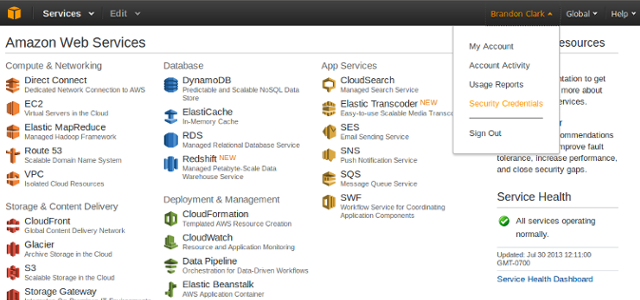
\includegraphics{getting_started-aws_security.png}

Under the ``Access Keys'' heading click the ``Create New Root Key''
button. You will be prompted to ``Download Key File'' which by default
is named \code{rootkey.csv}. Open this file to get the access-key and secret-
key for the environments.yaml configuration file.

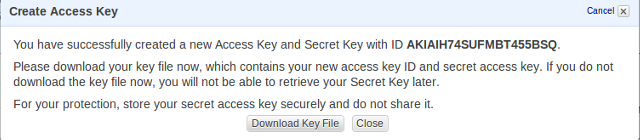
\includegraphics{getting_started-aws_keys.png}

The region: value corresponds to the AWS regions.


\chapter{Configuring for Windows Azure}
\label{config-azure:configuring-for-windows-azure}\label{config-azure:http-console-aws-amazon-com}\label{config-azure::doc}
This process requires you to have an Windows Azure account. If you
have not signed up for one yet, it can obtained at
\href{http://www.windowsazure.com/}{http://www.windowsazure.com/}.

You should start by generating a generic configuration file for Juju,
using the command:

\begin{Verbatim}[commandchars=\\\{\}]
juju generate-config
\end{Verbatim}

This will generate a file, environments.yaml , which will live in your
\textasciitilde{}/.juju/ directory (and will create the directory if it doesn't
already exist).

\begin{notice}{note}{Note:}
The above command will not overwrite your existing
environments.yaml file, or output to stdout. In order to see the
boilerplate environment.yaml on stdout you need to append the \code{-{-}show}
option. This is helpful if you have an existing environment.yaml and
just need to add a section. For example:
\end{notice}

\begin{Verbatim}[commandchars=\\\{\}]
juju generate-config --show
\end{Verbatim}

You can then copy and paste the needed section.

The generic configuration sections generated for Windows Azure will
look something like this:

\begin{Verbatim}[commandchars=\\\{\}]
azure:
  type: azure
  admin-secret: 35d65be36c72da940933dd02f8d7cef0
  \# Location for instances, e.g. West US, North Europe.
  location: West US
  \# http://msdn.microsoft.com/en-us/library/windowsazure
  \# Windows Azure Management info.
  management-subscription-id: 886413e1-3b8a-5382-9b90-0c9aee199e5d
  management-certificate-path: /home/me/azure.pem
  \# Windows Azure Storage info.
  storage-account-name: juju0useast0
  \# Public Storage info (account name and container name) denoting a public
  \# container holding the juju tools.
  \# public-storage-account-name: jujutools
  \# public-storage-container-name: juju-tools
  \# Override OS image selection with a fixed image for all deployments.
  \# Most useful for developers.
  \# force-image-name: b39f27a8b8c64d52b05eac6a62ebad85\_\_Ubuntu-13\_10-amd64-server-DEVELOPMENT-20130713-Juju\_ALPHA-en-us-30GB
  \# Pick a simplestreams stream to select OS images from: daily or released
  \# images, or any other stream available on simplestreams.  Leave blank for
  \# released images.
  \# image-stream: ""
  \# default-series: precise
\end{Verbatim}

This is the configuration environments.yaml file needed to run on
Windows Azure. You will need to set the \code{management-subscription-id},
\code{management-certificate-path}, and \code{storage-account-name}.

\begin{notice}{note}{Note:}
Other than \code{location} the other key vaule defaults are
recommended, but can be updated to your preference.
\end{notice}


\section{Config Values}
\label{config-azure:config-values}
Generate a new certificate for juju usage (or use an existing one).
Suggest to use a `Common Name' with `Juju' in it so its obvious in the
web UI later. Run the following commands on Ubuntu to generate a new
certificate:

\begin{Verbatim}[commandchars=\\\{\}]
openssl req -x509 -nodes -days 3650 -newkey rsa:2048 -keyout azure.pem -out azure.pem
openssl x509 -inform pem -in azure.pem -outform der -out azure.cer
chmod 600 azure.pem
\end{Verbatim}

Login to the Windows Azure console @ \href{https://manage.windowsazure.com}{https://manage.windowsazure.com}. From here you can gather the
following information:
\begin{itemize}
\item {} 
Settings Left Navigation: get the \code{SUBSCRIPTION ID} of the account
you upload to. This will be used for the \code{management-subscription-id}

\item {} 
Settings Left Navigation: ``upload'' the MyCert.cer file above (if you
created one). This is the certificate you used for the \code{management-
certificate-path}

\item {} 
Storage Left Navigation:
\begin{itemize}
\item {} 
Click New (bottom left)

\item {} 
Click Quick Create

\item {} 
Add a name in url (for example \code{juju0useast0}). This is the value to
be used for \code{storage-account-name}.

\item {} 
Select Location (for example: East US)

\item {} 
Select Subscription

\item {} 
Disable ``Enable Geo-Replication'' (not applicable)

\end{itemize}

\end{itemize}
\setbox0\vbox{
\begin{minipage}{0.95\linewidth}
\textbf{Note:}

\medskip


You must create the storage account in the same region/location
specified by the \code{location} key value. For example, if \code{location: West
US} is set then \code{storage-account-name:} must also have a storage set
up in \code{West US}. Failure to do so will result in a group affinity
error.
\end{minipage}}
\begin{center}\setlength{\fboxsep}{5pt}\shadowbox{\box0}\end{center}

Ensure the environments.yaml is configured with the above values and
save.


\chapter{Configuring for HPCloud}
\label{config-hpcloud:configuring-for-hpcloud}\label{config-hpcloud::doc}\label{config-hpcloud:videos}
You should start by generating a generic configuration file for Juju,
using the command:

\begin{Verbatim}[commandchars=\\\{\}]
juju generate-config
\end{Verbatim}

This will generate a file, environments.yaml , which will live in your
\textasciitilde{}/.juju/ directory (and will create the directory if it doesn't
already exist).

\begin{notice}{note}{Note:}
If you have an existing configuration, you can use {\color{red}\bfseries{}{}`{}`}juju
\end{notice}

generate-config --show{}`{}` to output the new config file, then copy and
paste relevant areas in a text editor etc.

The essential configuration sections for HPCloud look like this:

\begin{Verbatim}[commandchars=\\\{\}]
hpcloud:
  type: openstack
  use-floating-ip: false
  admin-secret: 139e8bee94d15bff96d91ab9c27e5efc
  \# Globally unique swift bucket name
  control-bucket: juju-9b53d6f5f45968d7c392a221f85fc8ae
  auth-url: https://region-a.geo-1.identity.hpcloudsvc.com:35357/v2.0/
  public-bucket-url: https://region-a.geo-1.objects.hpcloudsvc.com/v1/60502529753910
  auth-mode: userpass
  username: [your username]
  password: [password]
  tenant-name: [HP Cloud Project Name]
  region: [az-1.region-a.geo-1, az-2.region-a.geo-1, or az-3.region-a.geo-1]
\end{Verbatim}

The items highlighted are values you will need to enter, and are
explained below. You will find most of the relevant information on the
{\color{red}\bfseries{}{}`HP Cloud API Keys page{}`\_}
\begin{itemize}
\item {} 
\code{tenant-name:} For HPCloud, this is listed as the project name on
the {\color{red}\bfseries{}{}`''Manage Projects'' page{}`\_}.

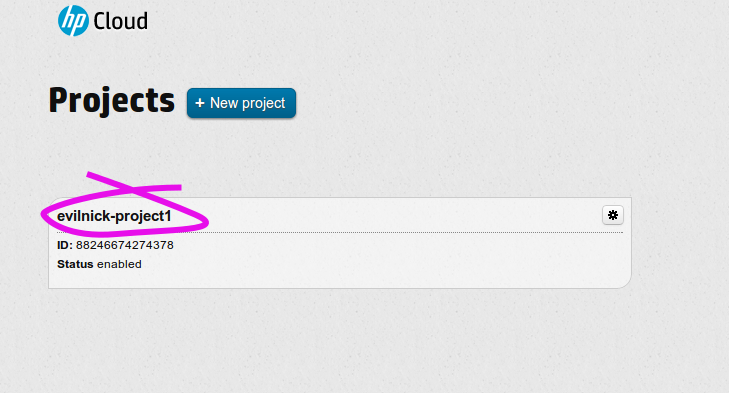
\includegraphics{getting_started-hpc-tenant.png}

\end{itemize}

You will find the following information on the {\color{red}\bfseries{}{}`HP Cloud API Keys
page for your account{}`\_}.
\begin{itemize}
\item {} 
\code{auth-url:} This is the keystone url for authentication. It is given
(on a region by region basis) under the heading ``Service Endpoints -
identity''

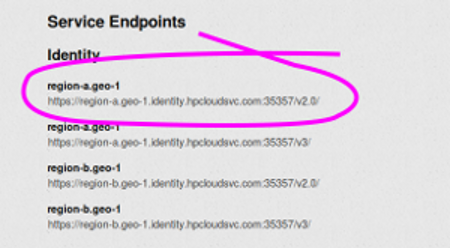
\includegraphics{getting_started-hpc-config1.png}

\item {} 
\code{region:} This is the longer format region name, given under the
headings for Block Storage and Compute sections.

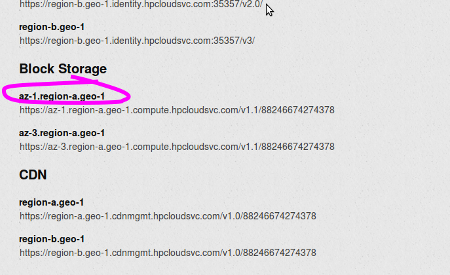
\includegraphics{getting_started-hpc-region.png}

\item {} 
\code{username:} Enter your HP Cloud login username.

\item {} 
\code{password:} Enter your HP Cloud login password.

\item {} 
\code{public-bucket-url:} Currently up to date tools are provided to HP
Cloud by a public bucket. If you're using your own imagemetadata you'd
change this URL to the bucket you've created.

\end{itemize}


\chapter{Configuring for OpenStack}
\label{config-openstack:configuring-for-openstack}\label{config-openstack::doc}\label{config-openstack:videos}
You should start by generating a generic configuration file for Juju,
using the command:

\begin{Verbatim}[commandchars=\\\{\}]
juju generate-config
\end{Verbatim}

This will generate a file, environments.yaml , which will live in your
\textasciitilde{}/.juju/ directory (and will create the directory if it doesn't
already exist).

\begin{notice}{note}{Note:}
If you have an existing configuration, you can use \code{juju
generate-config -{-}show} to output the new config file, then copy and
paste relevant areas in a text editor etc.
\end{notice}

The essential configuration sections for OpenStack look like this:

\begin{Verbatim}[commandchars=\\\{\}]
openstack:
  type: openstack
  \# Specifies whether the use of a floating IP address is required to give the nodes
  \# a public IP address. Some installations assign public IP addresses by default without
  \# requiring a floating IP address.
  \# use-floating-ip: false
  admin-secret: 13850d1b9786065cadd0f477e8c97cd3
  \# Globally unique swift bucket name
  control-bucket: juju-fd6ab8d02393af742bfbe8b9629707ee
  \# Usually set via the env variable OS\_AUTH\_URL, but can be specified here
  \# auth-url: https://yourkeystoneurl:443/v2.0/
  \# override if your workstation is running a different series to which you are deploying
  \# default-series: precise
  \# The following are used for userpass authentication (the default)
  auth-mode: userpass
  \# Usually set via the env variable OS\_USERNAME, but can be specified here
  \# username:
  \# Usually set via the env variable OS\_PASSWORD, but can be specified here
  \# password:
  \# Usually set via the env variable OS\_TENANT\_NAME, but can be specified here
  \# tenant-name:
  \# Usually set via the env variable OS\_REGION\_NAME, but can be specified here
  \# region:
\end{Verbatim}

\begin{notice}{note}{Note:}
At any time you can run \code{juju init -{-}show} to display the most
revent version of the environments.yaml template file, instead of
having it write to file.
\end{notice}

Remember to substitute in the parts of the snippet that are important
to you. If you are deploying on OpenStack the following documentation
might also be useful:

\href{https://help.ubuntu.com/community/UbuntuCloudInfrastructure}{Ubuntu Cloud Infrastructure}


\chapter{Configuring for MAAS}
\label{config-maas::doc}\label{config-maas:configuring-for-maas}\label{config-maas:videos}
Metal As A Service is software which allows you to deal with physical
hardware just as easily as virtual nodes. For more information about
MAAS, see \href{http://maas.ubuntu.com}{maas.ubuntu.com}

You should start by generating a generic configuration file for Juju,
using the command:

\begin{Verbatim}[commandchars=\\\{\}]
juju generate-config
\end{Verbatim}

This will generate a file, environments.yaml , which will live in your
\textasciitilde{}/.juju/ directory (and will create the directory if it doesn't
already exist).

\begin{notice}{note}{Note:}
If you have an existing configuration, you can use \code{juju
generate-config -{-}show} to output the new config file, then copy and
paste relevant areas in a text editor etc.
\end{notice}


\section{Get your API key}
\label{config-maas:get-your-api-key}
You'll need an API key from MAAS so that the Juju client can access
it. Each user account in MAAS can have as many API keys as desired.
One hard and fast rule is that you'll need to use a different API key
for each Juju environment you set up within a single MAAS cluster.

To get the API key:
\begin{enumerate}
\item {} 
Go to your MAAS preferences page, or go to your MAAS home page and
choose Preferences from the drop-down menu that appears when clicking
your username at the top-right of the page.

\item {} 
Optionally add a new MAAS key. Do this if you're setting up another
environment within the same MAAS cluster.

\item {} 
Copy the key value - you will need it shortly!

\end{enumerate}


\section{Edit or create the configuration}
\label{config-maas:edit-or-create-the-configuration}
Create or modify \code{\textasciitilde{}/.juju/environments.yaml} with the following
content:

\begin{Verbatim}[commandchars=\\\{\}]
maas:
  type: maas
  maas-server: 'http://xxyourMAASServernamexx:80/MAAS'
  maas-oauth: '\$MAAS\_API\_KEY'
  admin-secret: 'nothing'
  default-series: 'precise'
\end{Verbatim}

Substitute the API key from earlier into the \code{\$MAAS\_API\_KEY} slot. You
may need to modify the \code{maas-server} setting too; if you're running
from the maas package it should be something like
``\href{http://hostname.xxxx.yyy/MAAS}{http://hostname.xxxx.yyy/MAAS}''.


\chapter{Introduction}
\label{index:introduction}\label{index:videos}
This tutorial will show you how to get started with Juju, including
installing, configuring and bootstrapping a new Juju environment.
Before you start you will need:
\begin{itemize}
\item {} 
An Ubuntu, OSX or Windows machine to install the client on.

\item {} 
An environment which can provide a new server with an Ubuntu cloud
operating system image on-demand. This includes services such as
Amazon EC2, HP Cloud, an OpenStack installation, or your local machine

\item {} 
An SSH key-pair. If you have not already set one up, you need to
generate an appropriate keypair. On Linux and Mac OSX: \code{ssh-keygen -t
rsa -b 2048} On Windows: See the Windows instructions for SSH and
PuTTY

\end{itemize}


\chapter{Installation}
\label{index:installation}
To install Juju, you simply need to grab the latest juju-core package
from the PPA:
\begin{itemize}
\item {} 
\textbf{Ubuntu :}

\begin{Verbatim}[commandchars=\\\{\}]
sudo add-apt-repository ppa:juju/stable
sudo apt-get update \&\& sudo apt-get install juju-core
\end{Verbatim}

\item {} 
\textbf{Mac OSX :}

Juju is in \href{http://brew.sh/}{Homebrew}, to install do:

\begin{Verbatim}[commandchars=\\\{\}]
brew install juju
\end{Verbatim}

\item {} 
\textbf{Windows :}

Download and run the \href{https://launchpad.net/juju-core/1.16/1.16.2/+download/juju-setup-1.16.2-signed.exe}{Juju windows installer from here.}

\end{itemize}


\chapter{Configuring}
\label{index:configuring}
Now the Juju software is installed, it needs to be configured to use
your particular cloud provider. This is done by generating and editing
a file, \code{environments.yaml}, which will live in your \code{\textasciitilde{}/.juju/}
directory on Linux and OSX, \code{\%LOCALAPPDATA\%/Juju} on Windows. You can
generate the environments file manually, but Juju also includes a
boilerplate configuration option that will flesh out most of the file
for you and minimise the amount of work (and potential errors).

To generate an initial config file, you simply need to run:

\begin{Verbatim}[commandchars=\\\{\}]
juju generate-config
\end{Verbatim}

This command will cause a file to be written to your \textasciitilde{}/.juju directory
if an environments.yaml file does not already exist. It will also
create the \textasciitilde{}./juju directory if that does not exist.

This file will contain sample profiles for different types of cloud
services, but you will need to edit the files to provide specific
information for your cloud provider. Sections are created for Amazon
(AWS) services, HPCloud and a generic OpenStack instance (and for the
local provider if running on Linux). For more specifics on what needs
to be changed, see the relevant sections below.
\begin{itemize}
\item {} 
Configuring for Amazon AWS

\item {} 
\href{https://juju.ubuntu.com/config-azure.html}{Configuring for Windows Azure}

\item {} 
Configuring for HP Cloud

\item {} 
Configuring for OpenStack

\item {} 
Configuring for MAAS

\item {} 
\href{https://juju.ubuntu.com/config-local.html}{Configuring for LXC local provider (Linux)}

\end{itemize}


\chapter{Testing your setup}
\label{index:testing-your-setup}
Once you have installed and configured Juju, it is probably a good
idea to take it for a bit of a test drive and check that everything is
working as expected. Because Juju makes it really easy to deploy
services, this is actually quick and straightforward.

The first thing to do is set up a bootstrap environment. This is an
instance in the cloud that Juju will use to deploy and control other
services with. It will be created according to the configuration you
have provided, and your SSH key will automatically be uploaded so that
Juju can communicate securely with the bootstrap instance.

\begin{Verbatim}[commandchars=\\\{\}]
juju bootstrap
\end{Verbatim}

\begin{notice}{note}{Note:}
If you have multiple environments configured, you can choose
which one to address with a particular command by adding the \code{-e}
switch followed by the environment name, E.g. \code{-e hpcloud}.
\end{notice}

You may have to wait a few moments for this command to return, as it
needs to perform various tasks and contact your cloud provider.

Assuming it returns successfully (otherwise see common error messages
and what to do about them), we can now deploy some services and
explore the basic operations of Juju.

To start with, we will deploy Wordpress, by running this command:

\begin{Verbatim}[commandchars=\\\{\}]
juju deploy wordpress
\end{Verbatim}

Now juju will fetch the Wordpress charm and use it, through the
bootstrap instance to request and deploy whatever resources it needs
to set up this service.

Wordpress needs a database though, so we will also deploy one of
those:

\begin{Verbatim}[commandchars=\\\{\}]
juju deploy mysql
\end{Verbatim}

Once again, juju will do whatever is necessary to deploy this service
for you, and it may take some time for the command to return.

\begin{notice}{note}{Note:}
If you want to get more information on what is actually
happening, or to help resolve problems, you can add the -v switch to
the juju command to get verbose output.
\end{notice}

Although we have deployed Wordpress and a MySQL database, they are not
linked together in any way yet. To do this we should run:

\begin{Verbatim}[commandchars=\\\{\}]
juju add-relation wordpress mysql
\end{Verbatim}

This command uses information provided by the relevant charms to
associate these services with each other in whatever way makes sense.
There is much more to be said about linking services together which is
covered in the juju command documentation, but for the moment, we just
need to know that it will link these services together.

In order to make our Wordpress public, we now need to expose this
service:

\begin{Verbatim}[commandchars=\\\{\}]
juju expose wordpress
\end{Verbatim}

This service will now be configured to respond to web requests, so
visitors can see it. But where exactly is it? If we run the juju
status command, we will be able to see what services are running, and
where they are located.

\begin{Verbatim}[commandchars=\\\{\}]
juju status
\end{Verbatim}

The output from this command should look something like this:

\begin{Verbatim}[commandchars=\\\{\}]
machines:
  "0":
    agent-state: started
    agent-version: 1.10.0
    dns-name: ec2-50-16-167-135.compute-1.amazonaws.com
    instance-id: i-781bf614
    series: precise
  "1":
    agent-state: started
    agent-version: 1.10.0
    dns-name: ec2-23-22-225-54.compute-1.amazonaws.com
    instance-id: i-9e8927f6
    series: precise
  "2":
    agent-state: started
    agent-version: 1.10.0
    dns-name: ec2-54-224-220-210.compute-1.amazonaws.com
    instance-id: i-5c440436
    series: precise
services:
  mysql:
    charm: cs:precise/mysql-18
    exposed: false
    relations:
      db:
      - wordpress
    units:
      mysql/0:
        agent-state: started
        agent-version: 1.10.0
        machine: "1"
        public-address: ec2-23-22-225-54.compute-1.amazonaws.com
  wordpress:
    charm: cs:precise/wordpress-12
    exposed: true
    relations:
      db:
      - mysql
      loadbalancer:
      - wordpress
    units:
      wordpress/0:
        agent-state: started
        agent-version: 1.10.0
        machine: "2"
        public-address: ec2-54-224-220-210.compute-1.amazonaws.com
\end{Verbatim}

There is quite a lot of information here. the first section, titled
machines: , details all the instances which are currently running. For
each you will see the version of Juju they are running, their
hostname, instance id and the series or version of Ubuntu they are
running.

After that, the sections list the services which are currently
deployed. The information here differs slightly according to the
service and how it is configured. It will however, always list the
charm that was used to deploy the service, whether it is exposed or
not, its address and whatever relationships exist.

From this status readout, we can see that wordpress is exposed and
ready. If we simply copy the address into a web browser, we should be
able to see it running

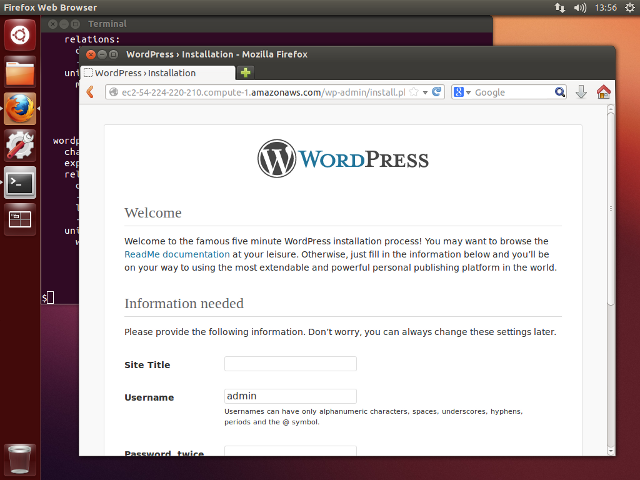
\includegraphics{getting_started-wordpress.png}

Congratulations, you have just deployed a service with Juju!

Now you are ready to deploy whatever service you really want from the
100s available at the \href{http://jujucharms.com}{Juju Charm Store.}

To remove all current deployments and clear up everything in your
cloud, you can run the command:

\begin{Verbatim}[commandchars=\\\{\}]
juju destroy-environment
\end{Verbatim}

This will remove everything, including the bootstrap node.

To learn more about charms, including configuring options and managing
running systems, you should continue to \href{https://juju.ubuntu.com/./charms.html}{read the charm
documentation.}



\renewcommand{\indexname}{Index}
\printindex
\end{document}
